\begin{figure}[!htbp]\centering
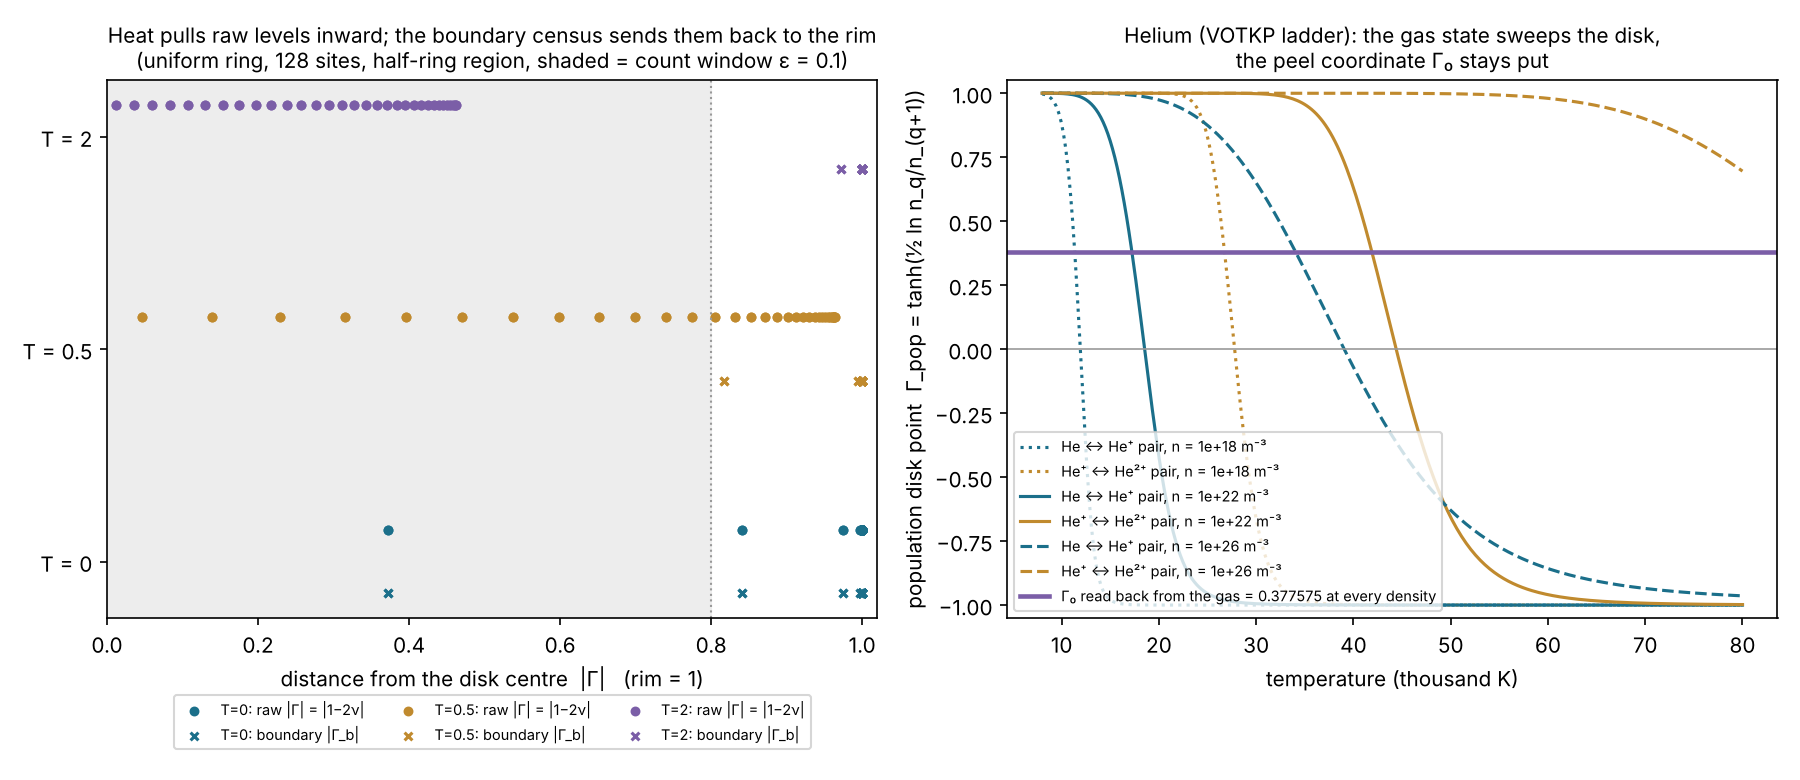
\includegraphics[width=\textwidth]{../figures/fig02_boundary_and_gas.png}
\caption{Left: heat pulls raw census levels toward the centre of the disk; the boundary coordinate $|\Gamma_b|$ counts only strengths that cross the cut, and a zero count at $T=0.5$ still has $\Tr X_A=0.170835$ below the window. Right: helium's charge-state pairs sweep the disk as the gas changes, while $\Gamma_0$ read back from the gas stays at $0.377575$ (ideal Saha model, ground-state partitions).}
\label{fig:boundary}
\end{figure}

\section{One chart for all of it}\label{sec:chart}
\begin{theorem}[peel steps add like velocities; VOTKP Theorem 15.1]\label{thm:add}
For a positive ladder $I_0,\dots,I_n$ with steps $\Gamma_k=\tanh(\tfrac12\ln(I_{k+1}/I_k))$, the composite of a block of steps is $\Gamma_{j\to l}=\Gamma_j\oplus\Gamma_{j+1}\oplus\dots\oplus\Gamma_{l-1}$, with $u\oplus v=(u+v)/(1+uv)$. \grade{T}\grade{L}
\end{theorem}
\begin{proof}
$\ln(I_l/I_j)=\sum_k\ln(I_{k+1}/I_k)$, and $\tanh(a+b)=\tanh a\oplus\tanh b$ (A.8).
\end{proof}
This is Einstein's addition of collinear velocities; the half-rapidities add. On the Smith disk read as the Poincaré disk the peel is a walk along a geodesic diameter whose hyperbolic lengths, $2\operatorname{artanh}|\Gamma|$, add (VOTKP Corollary 15.2) \grade{T}. The composite forgets the order of its steps; the resolved ladder keeps it.

\paragraph{Matter's census ladder is a peel ladder.} On the transverse-field Ising chain ($c=\tfrac12$) the single-particle entanglement energies are odd multiples $\varepsilon_0,3\varepsilon_0,5\varepsilon_0,\dots$ of one spacing (\emph{Matter at a Scale}, LADDER-C12-01). By Theorem~\ref{thm:add} the levels then satisfy $\Gamma_{j+1}=\Gamma_j\oplus\tanh\varepsilon_0$: one constant peel step. Measured residuals are $8.0\times10^{-6}$, $5.5\times10^{-6}$, $3.2\times10^{-6}$ at $\xi=20.5$, $50.5$, $125.5$, and the ladder's own uniformity error falls $0.022$, $0.011$, $0.0062$ \grade{V} (script \texttt{s02}). Near the rim the disk compresses differences, so the informative number is the uniformity error in rapidity.

Figure~\ref{fig:hero} places every reading of this paper on the one disk at its signed value. Real ratios sit on the real diameter; the bound nuclei, read in VOTKP's order $z=S_{\mathrm{next}}/S_{\mathrm{first}}$, have $z<1$ and so lie on the negative half, and the unbound ones lie past $+1$.

\begin{figure}[!htbp]\centering
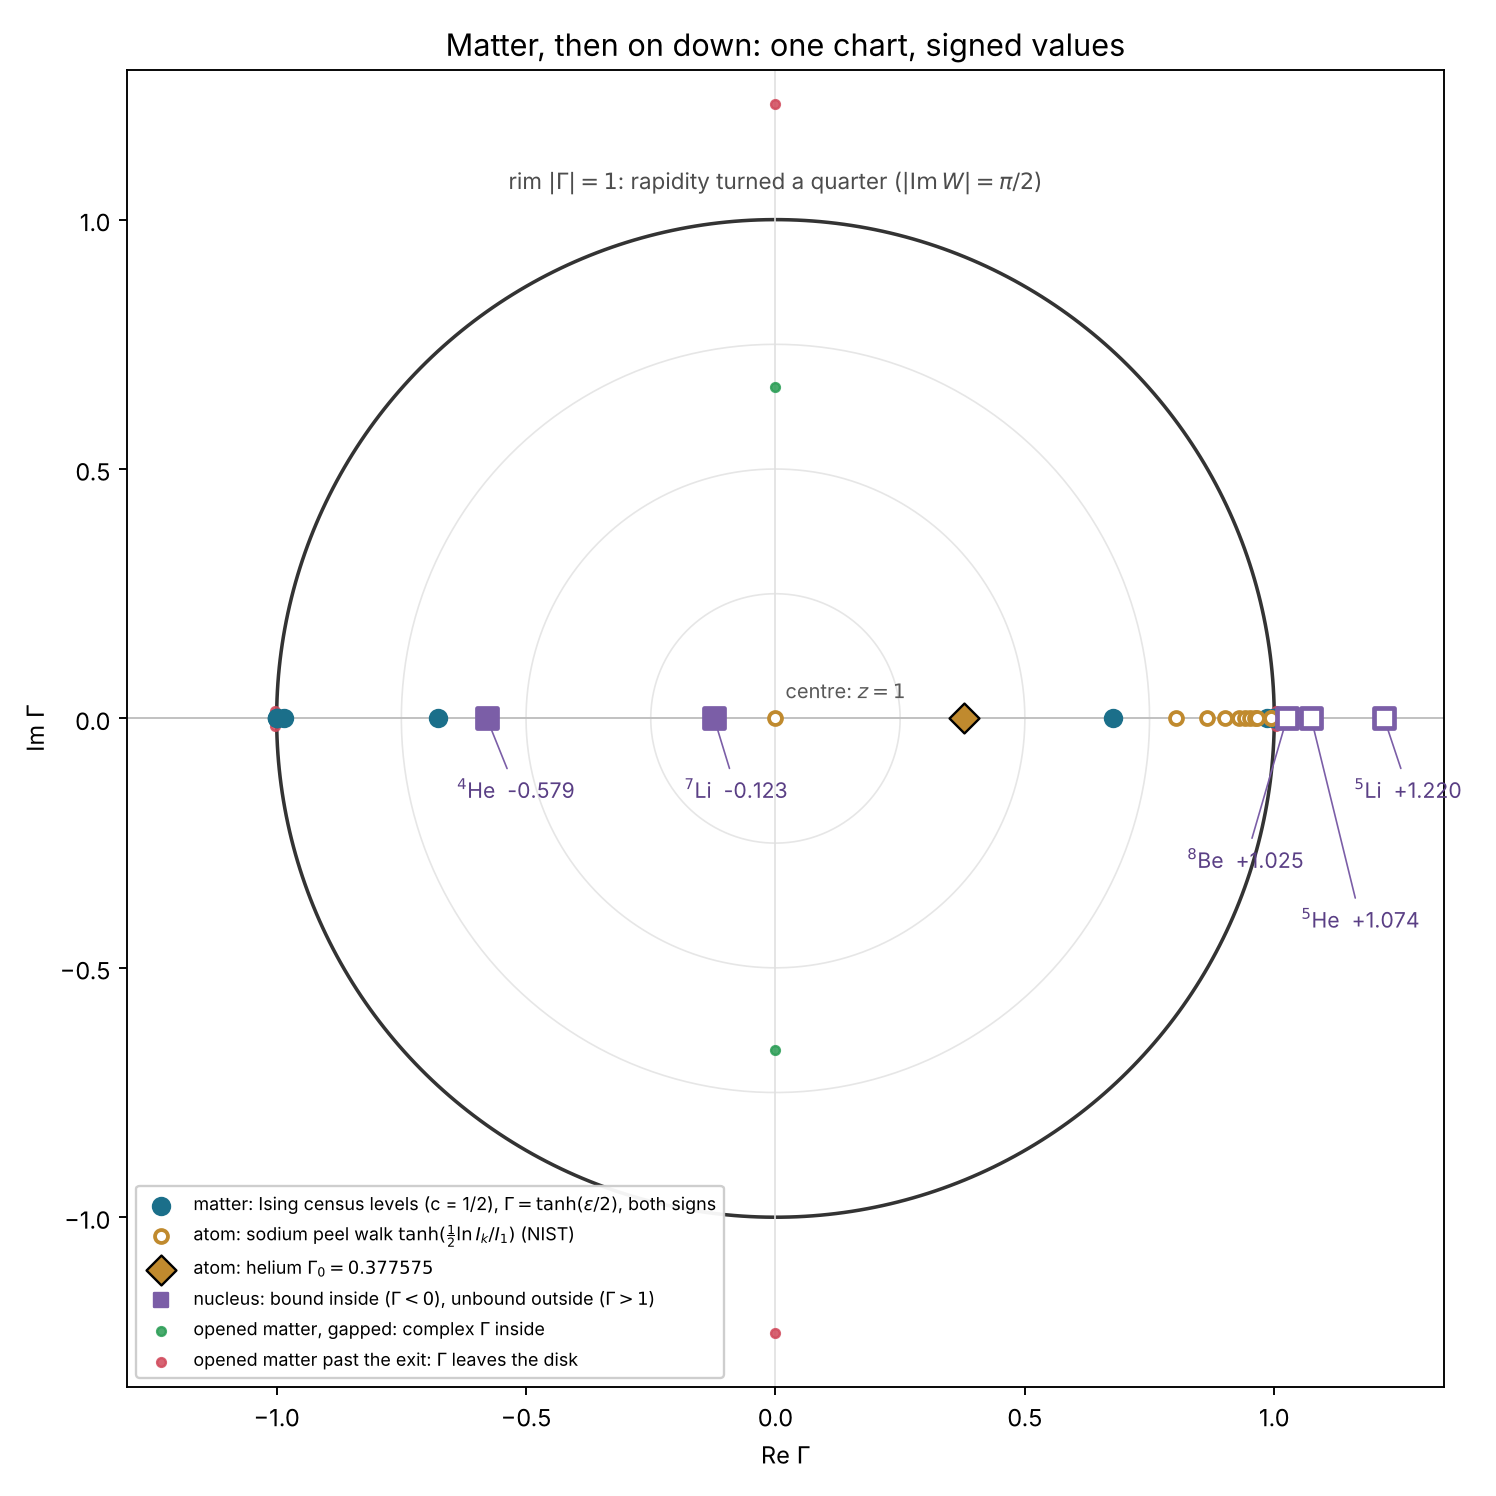
\includegraphics[width=0.86\textwidth]{../figures/fig03v4_one_chart.png}
\caption{One chart, every scale, signed. Blue: the Ising census ladder $\Gamma=\tanh(\varepsilon/2)$ on both signs. Gold: sodium's peel walk $\tanh(\frac12\ln I_k/I_1)$ from the NIST thresholds, ending at $0.9938$, and helium's $\Gamma_0$. Purple: nuclear separation-energy peels in the order $z=S_{\mathrm{next}}/S_{\mathrm{first}}$ (NUBASE2020); ${}^7$Li and ${}^4$He inside at $-0.123$ and $-0.579$, the unbound mass-5 and mass-8 gaps outside. Green and red: census levels of the opened non-Hermitian SSH chain ($u=0.5$) before ($v=0.30$) and past ($v=0.49$) its exit.}
\label{fig:hero}
\end{figure}

\section{The disk as a reflection chart}\label{sec:reflection}
The Smith chart was built for reflection. The black-hole paper of the author (\emph{Beyond the Event Horizon}, ed.~10, §§5, 7, 8) places three boundary readings on the same disk, and each lends the matter coordinate a meaning it did not have from occupations alone. They are different normalised impedances on one chart; their relative positions are not a physical identification (Figure~\ref{fig:reflection}).

\subsection{A step in spectral gap reflects with the peel coordinate}
On a projector family with pullback metric $g=a(y)\,dx^2+b(y)\,dy^2$ ($a=g_\parallel$, $b=g_\perp$), a wave $\psi=e^{ipx}u(y)$ of the Laplace–Beltrami operator at frequency $\omega$ conserves the Clairaut constant $C=a\sin^2\theta$ and carries the admittance $Y=\omega\sqrt{a-C}=\omega\sqrt{g_\parallel}\cos\theta$. At a step $(a_1,b_1)\to(a_2,b_2)$,
\begin{equation}
\Gamma=\frac{\sqrt{a_1-C}-\sqrt{a_2-C}}{\sqrt{a_1-C}+\sqrt{a_2-C}},\qquad \sqrt{a_2-C}\to i\sqrt{C-a_2}\ \text{when}\ C>a_2,
\label{eq:step}
\end{equation}
so $g_\perp$ drops out, and $|\Gamma|=1$ exactly beyond the geodesic turning point $a_2=C$ \grade{T} (ed.~10, eqs.~47–49). At normal incidence $C=0$ and $\Gamma=\tanh(\tfrac12\ln\sqrt{a_1/a_2})$. When the index is set by the spectral gap at fixed coupling, as on the IQGT family $\Sigma=\cos3x\,\sigma_x+\sin3x\,\sigma_y+2.5y\,\sigma_z$ where $g_\parallel\Delta^2=9$ \grade{T} (\emph{Intrinsic QGT}, §8.6), $\sqrt{g_\parallel}\propto1/\Delta$ and
\begin{equation}
\Gamma=\frac{\Delta_2-\Delta_1}{\Delta_2+\Delta_1}=\tanh\Big(\tfrac12\ln\frac{\Delta_2}{\Delta_1}\Big):
\label{eq:gapstep}
\end{equation}
the peel coordinate, now as the reflection of a wave at a change of gap \grade{T}. Script \texttt{s13} solves the matching problem directly (continuity of $u$ and $u'$ for $u''+\omega^2n^2u=0$, $n=1/\Delta$) on 200 random steps and recovers \eqref{eq:gapstep} to $3.3\times10^{-16}$ \grade{V}. The black-hole paper's own sharp-step matching reproduces \eqref{eq:step} to $1.7\times10^{-11}$ on 400 random steps, 89 beyond the turning point. Its preregistered Richardson gate for smooth steps failed (residual $7.4\times10^{-4}$ against $10^{-5}$), and the first-order limit was then tested directly with its own condition. A polar stratum is a perfect mirror there, $|r|=1$ to $2\times10^{-16}$ \grade{V}\grade{S}.

So the atom's peel and a gap step are one formula: successive removal thresholds are ratios of gaps measured from the continuum, and $\Gamma$ is what a wave crossing from one gap to the next would see reflected.

\subsection{The centre is a matched load; the inside is passive}
\begin{proposition}[Schur–Cayley boundary; ed.~10, Prop.~13]\label{prop:schurcayley}
Let $L$ be passive, $\mathrm{Herm}\,L=\tfrac12(L+L^*)\ge0$, split into boundary $b$ and interior $i$ with $L_{ii}$ invertible. The boundary impedance $Z_b=L_{bb}-L_{bi}L_{ii}^{-1}L_{ib}=W^*LW$, $W=\begin{pmatrix}I\\-L_{ii}^{-1}L_{ib}\end{pmatrix}$, has $\mathrm{Herm}\,Z_b=W^*(\mathrm{Herm}\,L)W\ge0$, and $S_b=(Z_b-I)(Z_b+I)^{-1}$ satisfies
\[
I-S_b^*S_b=4(WV_b)^*(\mathrm{Herm}\,L)(WV_b)\ge0,\qquad V_b=(Z_b+I)^{-1},
\]
so $\|S_b\|\le1$, with $S_b=0$ exactly for the matched load $Z_b=I$. No normality is assumed. \grade{T}
\end{proposition}
\begin{proof}
$W^*LW=L_{bb}-L_{bi}L_{ii}^{-1}L_{ib}-L_{bi}L_{ii}^{-1}L_{ib}+L_{bi}L_{ii}^{-1}L_{ii}L_{ii}^{-1}L_{ib}=Z_b$, and taking Hermitian parts commutes with the congruence. With $S_b=(Z_b-I)V_b$, $I-S_b^*S_b=V_b^*[(Z_b+I)^*(Z_b+I)-(Z_b-I)^*(Z_b-I)]V_b=2V_b^*(Z_b+Z_b^*)V_b=4V_b^*(\mathrm{Herm}\,Z_b)V_b$, and substitute $\mathrm{Herm}\,Z_b$.
\end{proof}
The inside of the disk is the passive boundary; the centre is the load that returns nothing; the rim is total reflection. Through the membrane paradigm the stretched horizon has surface resistivity $4\pi$ in Gaussian units, the impedance of empty space $\mu_0c=376.73\,\Omega$, so normalised by the vacuum impedance the horizon surface is $Z_b=1$, $S_b=0$: the centre of the chart \grade{S} (sourced; ed.~10 §5.2). The match belongs to the horizon surface, not to the hole seen from far away: the potential barrier outside reflects long-wavelength radiation. Matter's unbound nuclei (§\ref{sec:nucleus}) lie outside the rim, beyond what any passive boundary can reach.

\subsection{The outside record of a Hawking fermion pair}
\begin{proposition}[the fermion record; ed.~10, eqs.~38–39]\label{prop:hawking}
For a Dirac pair $\cos r|00\rangle+e^{i\phi}\sin r|11\rangle$ with $\tan^2r=e^{-\hbar\omega/k_BT_H}$, the outside occupation is $C=\sin^2r$, and
\[
\tau=\log\frac{\det(I-C)}{\det C}=\log\frac{P(\mathrm{empty})}{P(\mathrm{full})}=\frac{\hbar\omega}{k_BT_H},\qquad \Gamma=1-2C=\tanh\frac{\hbar\omega}{2k_BT_H},
\]
for every pair phase $\phi$; for independent modes $\tau=\sum_k\hbar\omega_k/k_BT_H$. \grade{T}
\end{proposition}
\begin{proof}
The partial trace over the inside mode removes the coherence and leaves occupation $\sin^2r$, independent of $\phi$. Then $(1-C)/C=\cot^2r=e^{\hbar\omega/k_BT_H}$; take logs and apply Proposition~\ref{prop:bridge}.
\end{proof}
Script \texttt{s13} takes the partial trace at six frequencies and seven phases and recovers both identities to $5\times10^{-16}$ \grade{V}. The identity is the logarithm of a Boltzmann factor; what it adds is the reading. The outside record is the matter offset of §\ref{sec:ledger}: it sits at $\Gamma=\tanh(\hbar\omega/2k_BT_H)$, reaches the centre where the matched horizon sits only at zero frequency, and particle–hole exchange $C\mapsto1-C$ sends $\Gamma\mapsto-\Gamma$. It fixes only the ratio $\omega/T_H$, never an absolute scale, which is §\ref{sec:size}'s zero and span again; and the phase $\phi$ that decides what the pair does next never enters it, which is Proposition~\ref{prop:joint}'s lesson at a horizon \grade{H}\grade{S}. The construction needs $0<C<I$, so it holds for fermion modes; the bosonic pair has no full state.

\begin{figure}[!htbp]\centering
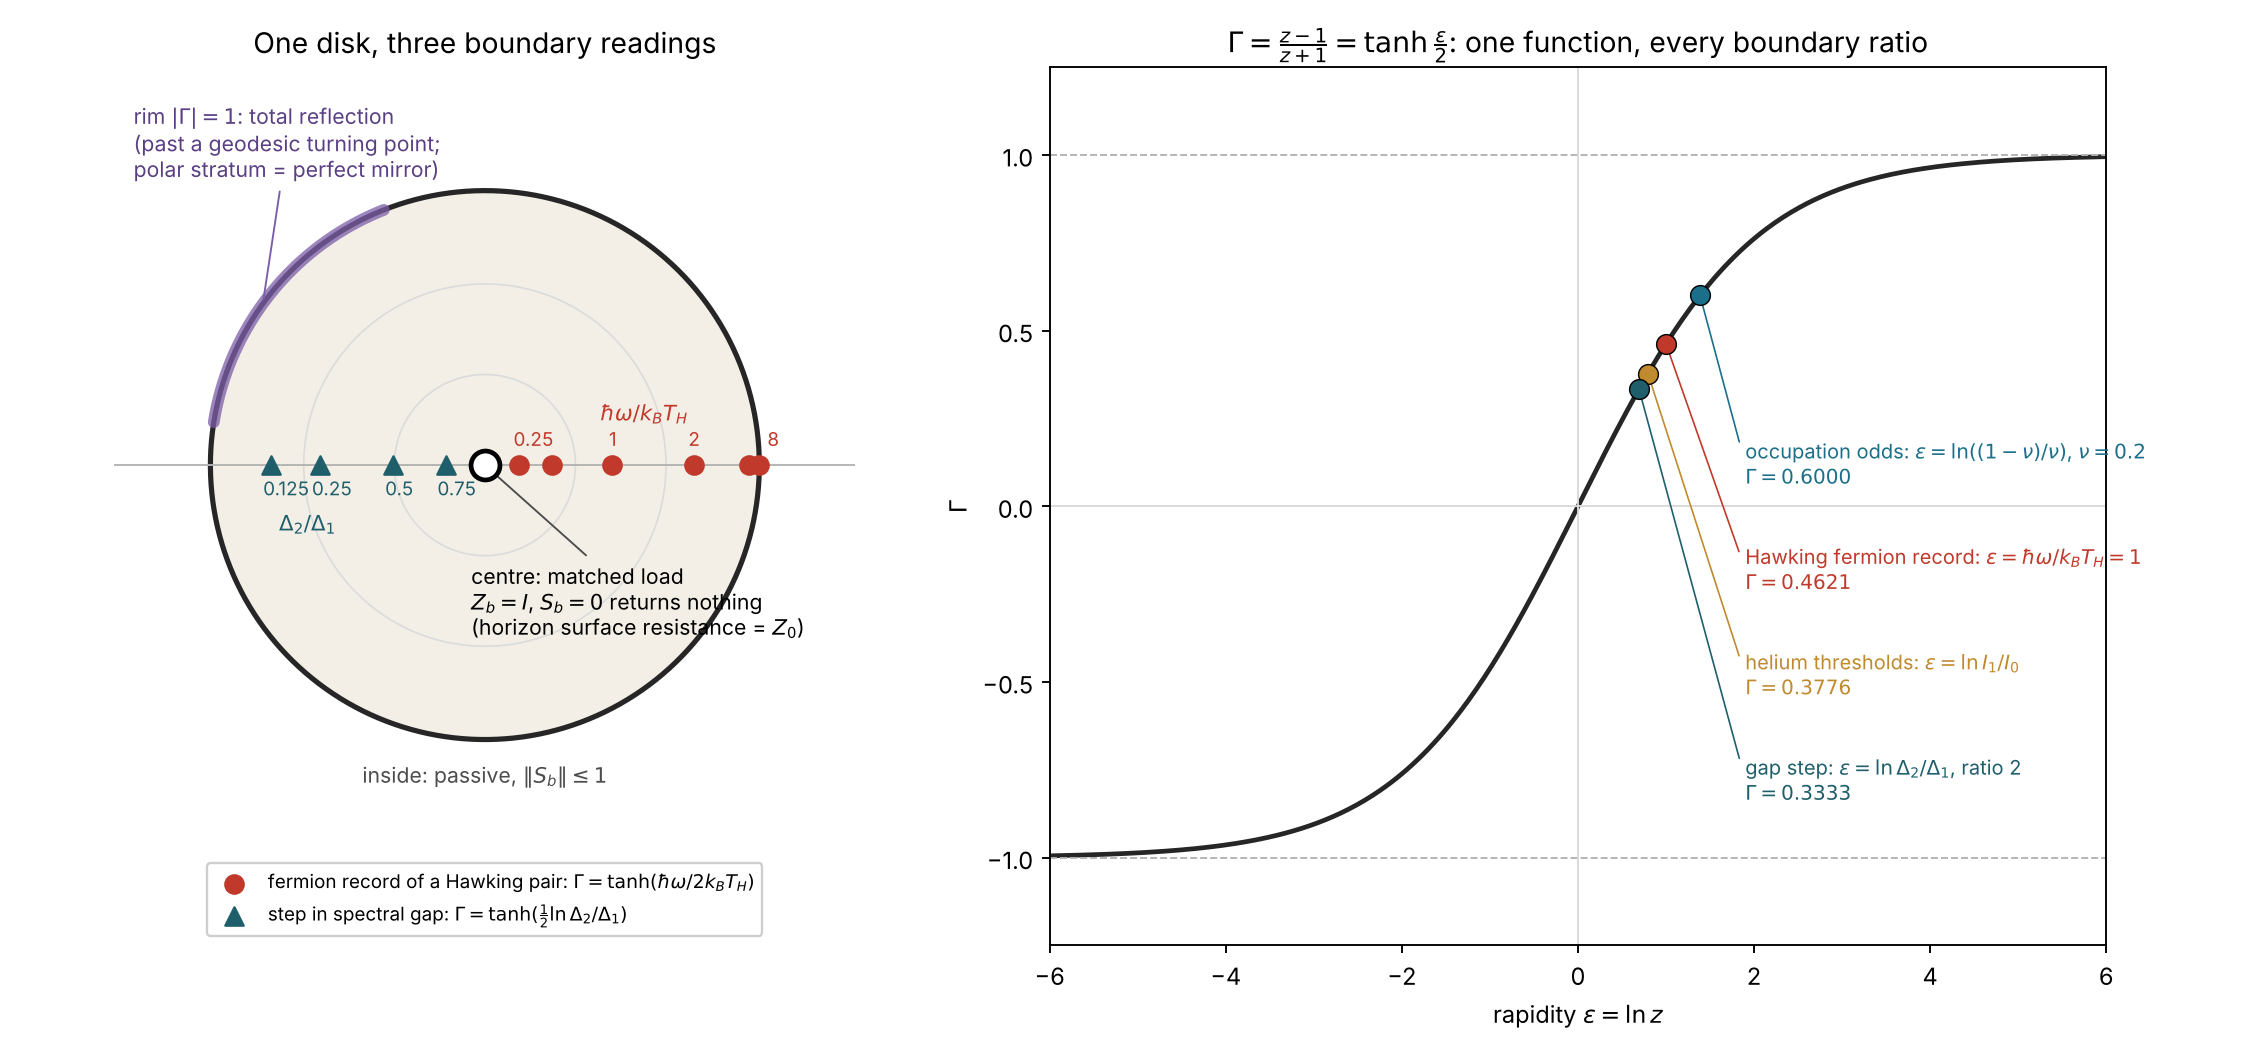
\includegraphics[width=\textwidth]{../figures/fig04_reflection_chart.png}
\caption{Left: one disk carrying three boundary readings: the matched load at the centre, total reflection on the rim, the Hawking fermion record $\tanh(\hbar\omega/2k_BT_H)$ (red, labelled by $\hbar\omega/k_BT_H$) and the reflection at a step in spectral gap $\tanh(\frac12\ln\Delta_2/\Delta_1)$ (green, labelled by $\Delta_2/\Delta_1$). Right: the single curve $\Gamma=\tanh(\varepsilon/2)$ with four readings of the rapidity marked at their real values.}
\label{fig:reflection}
\end{figure}

\section{The atom}\label{sec:atom}
For an atom the ratio is between successive relaxed removal thresholds, $z_q=I_{q+1}/I_q$, and every step lies on the positive real radius (VOTKP §8, Theorem 8.1 chart). The index labels successive charge-state removals, not excitations within one fixed-charge Hamiltonian.

\begin{theorem}[anchored coordinate equivalence]\label{thm:anchor}
For $Z\ge1$ the map $I=(I_0,\dots,I_{Z-1})\mapsto(I_0,\Gamma_0,\dots,\Gamma_{Z-2})$ is a bijection from $(0,\infty)^Z$ onto $(0,\infty)\times(-1,1)^{Z-1}$, with inverse $I_q=I_0\prod_{j<q}(1+\Gamma_j)/(1-\Gamma_j)$. A common scale $I\mapsto cI$ leaves every $\Gamma_q$ unchanged; two ladders have the same ratio vector iff they differ by one positive scale; and the anchored vector fixes every binding sum $B_q=\sum_{j\ge q}I_j$. \grade{T}\grade{L}
\end{theorem}
\begin{proof}
For $a,b>0$, $-1<(b-a)/(b+a)<1$ and $(1+\Gamma)/(1-\Gamma)=b/a$; adjacent ratios telescope. Conversely every factor of the inverse is positive for $\Gamma_j\in(-1,1)$. Common scaling cancels in each ratio; equal ratios give $I'_q/I_q=I'_0/I_0$ by induction.
\end{proof}
Any function of the complete ladder is a function of the anchored vector and conversely: the coordinate changes conditioning and representation, never information. Neither representation knows a specimen's temperature, density, partition weights, matrix elements or preparation (§\ref{sec:gas}).

Helium's two thresholds, $24.587389011$ and $54.4177655282$\,eV, give $\Gamma_0=0.37757506698375$ and a binding sum of $79.0051545392$\,eV \grade{lit}\grade{V}. VOTKP Theorem 15.4 (scale blindness) is the atomic form of §\ref{sec:size}: multiplying every mass of a nonrelativistic Coulomb system by $\lambda$ scales every energy by $\lambda$ and leaves every ratio fixed, so the peel coordinate is blind to which particle carries the charge except through charges, mass ratios and statistics \grade{T} (A.9). The coordinate needs a physical zero: removal energies are measured from the continuum, which is why the ratio means something, and why quantum-dot addition spectra, which can be moved up or down, have no peel (VOTKP §15.3).

Sodium's eleven thresholds walk from the centre to $\Gamma=0.9938$ along one diameter (Figure~\ref{fig:hero}); shell jumps are the long strides. For a helium-like ion of charge $Z\ge2$ the last peel step is, to first order in the electron repulsion, $\Gamma=5/(8Z-5)\to5/(8Z)$ \grade{T}\grade{L} (A.10). The middle of the peel follows the Thomas–Fermi law with $\Gamma_k\to\tanh(\tfrac23\ln\tfrac{k+1}{k})\approx2/(3k)$, cited in VOTKP §15.11 \grade{lit}.

\section{Gas}\label{sec:gas}
\emph{Matter at a Scale} §4 makes gas the gapless phase: the census floods, directions are free and failures are non-modal. On the disk the gas state is a layer that can be varied freely while an atomic record survives it. This section proves how much of the atom the gas carries, and what the gas must supply before the atom can be read back out. The model is the ideal, nonrelativistic, thermodynamic-equilibrium Saha gas of a pure species; mixtures, external electrons and non-LTE kinetics need other closures.

\subsection{One neutral state}
Fix $Z\ge1$, a nucleus density $N>0$ and positive coefficients $S_0,\dots,S_{Z-1}$ (number-density units). The finite Saha model is $n_{q+1}/n_q=S_q/x$, $\sum_qn_q=N$, $x=\sum_qqn_q$, with $x=n_e>0$. Set $a_0=1$, $a_q=\prod_{j<q}S_j$, $W(x)=\sum_qa_qx^{-q}$, $p_q=a_qx^{-q}/W$, $\mu=\sum qp_q$, $V=\sum(q-\mu)^2p_q$. Every population is positive, $0<\mu<Z$, $V>0$, and neutrality is $x=N\mu(x)$.

\begin{lemma}[exponential family]\label{lem:expfam}
With $y=\log x$: $dp_q/dy=p_q(\mu-q)$, $d\mu/dy=-V$, and $\frac{d}{dy}\mathbb E[f(q)]=-\mathrm{Cov}(f(q),q)$. \grade{T}
\end{lemma}
\begin{proof}
$dW(e^y)/dy=-\mu W$; differentiate $\log p_q$; multiply by $q$ or $f$ and sum.
\end{proof}

\begin{theorem}[a unique neutral gas]\label{thm:saha}
The model has exactly one positive solution, with $0<x<NZ$; it is the unique positive root of $P(x)=\sum_qa_qx^{Z-q+1}-N\sum_qqa_qx^{Z-q}$, of degree $Z+1$. For helium, with $u=x/N$, $\alpha=S_0/N$, $\beta=S_1/N$: $u^3+\alpha u^2+(\alpha\beta-\alpha)u-2\alpha\beta=0$, $0<u<2$. \grade{T}\grade{L}(three charges)
\end{theorem}
\begin{proof}
$F(x)=x-N\mu(x)$ has $F'=1+NV/x>1$; as $x\downarrow0$, $p_Z\to1$ and $F\to-NZ<0$; at $x=NZ$, $\mu<Z$ so $F>0$. Strict monotonicity gives one root; ratios and normalisation fix the populations.
\end{proof}

\begin{theorem}[how the neutral gas responds]\label{thm:response}
At fixed coefficients,
\[
\frac{d\log x}{d\log N}=\frac{\mu}{\mu+V}\in(0,1),\qquad\frac{d\mu}{d\log N}=-\frac{\mu V}{\mu+V}<0,\qquad\frac{d\log p_q}{d\log N}=(\mu-q)\frac{\mu}{\mu+V},
\]
and every upper tail $\Pr(q\ge r)$ falls with density. If $\theta$ varies the coefficients with $h_q=\partial_\theta\log a_q$ and $C_h=\mathrm{Cov}_p(q,h_q)$, then $\partial_\theta\log x=C_h/(\mu+V)$, $\partial_\theta\mu=\mu C_h/(\mu+V)$, $\partial_\theta p_q=p_q[h_q-\mathbb E h-(q-\mu)C_h/(\mu+V)]$; raising any single $S_r$ raises the mean charge. With $T$-independent partition weights, $d\log x/d\log T=\mathrm{Cov}(q,\tfrac32q+E_q/k_BT)/(\mu+V)>0$ with $E_q=\sum_{j<q}I_j$, and at fixed $T,N,U$, $\partial\mu/\partial I_r=-\mu\,\mathrm{Cov}(q,\mathbf 1_{q>r})/(k_BT(\mu+V))<0$. \grade{T}
\end{theorem}
\begin{proof}
Differentiate $x=N\mu(x)$: $dx/dN=\mu/(1+NV/x)=\mu^2/(\mu+V)$. Lemma~\ref{lem:expfam} gives the populations. For an increasing indicator $f$, $\mathrm{Cov}(f(q),q)=\tfrac12\sum_{i,j}p_ip_j(f(i)-f(j))(i-j)>0$. At fixed $x$, $\partial_\theta p_q=p_q(h_q-\mathbb Eh)$, so $\partial_\theta\mu=C_h$ at fixed $x$; the change through $x$ adds $-V\partial_\theta\log x$, and neutrality gives $\partial_\theta\mu=\mu\partial_\theta\log x$. For temperature, $a_q=(2/\lambda_e^3)^q(U_q/U_0)e^{-E_q/k_BT}$ has $h_q=3q/2+E_q/k_BT$ with positive increments $3/2+I_q/k_BT$.
\end{proof}
With temperature-dependent partitions the derivative gains $d\log(U_q/U_0)/d\log T$ and positivity needs an extra condition.

The physical coefficients are $S_q(T)=\frac{2U_{q+1}(T)}{\lambda_e(T)^3U_q(T)}e^{-I_q/k_BT}$, $\lambda_e=h/\sqrt{2\pi m_ek_BT}$, and by Theorem~\ref{thm:anchor}
\[
S_q(T)=\frac{2U_{q+1}(T)}{\lambda_e(T)^3U_q(T)}\exp\Big[-\frac{I_0}{k_BT}\prod_{j<q}\frac{1+\Gamma_j}{1-\Gamma_j}\Big]:
\]
Saha with a reconstructed threshold input, not a new ionisation law \grade{T}. It exposes the inputs the gas needs beyond the peel: the absolute thermal ratio $I_0/k_BT$, the density relative to $\lambda_e^3$, internal partition ratios, and a justified equilibrium.

\begin{theorem}[scaling and what the atom alone cannot know]\label{thm:scaling}
(i) $S_q\mapsto cS_q$, $N\mapsto cN$ preserves every charge fraction and sends $x\mapsto cx$. (ii) $m_e\mapsto am_e$, $T\mapsto bT$, $I_q\mapsto bI_q$ with partition ratios held, and $N\mapsto(ab)^{3/2}N$, preserve all populations. (iii) No function of the complete anchored threshold record determines the mean charge for all densities at fixed $T,U,m_e$; and no function of the unanchored ratio vector determines it even at fixed $T,N,U,m_e$. \grade{T}
\end{theorem}
\begin{proof}
(i) Ratios $S_q/x$ and neutrality are preserved; Theorem~\ref{thm:saha} gives uniqueness. (ii) $S'_q=(ab)^{3/2}S_q$, then (i). (iii) By Theorem~\ref{thm:response} the mean depends strictly on $N$; common threshold scaling fixes the ratio vector and changes the mean through $\partial\mu/\partial I_r<0$.
\end{proof}
The missing absolute anchor is physically consequential: common scaling of every threshold leaves every $\Gamma_q$ fixed and changes the gas. At nucleus density $10^{22}\,\mathrm{m^{-3}}$, with helium's ground partitions $(1,2,1)$, the neutral fraction is $0.999374$, $0.289781$ and $8.73350\times10^{-6}$ at $10^4$, $2\times10^4$ and $5\times10^4$\,K while $\Gamma_0$ stays at $0.377575$: the atomic record alone does not determine a gas population \grade{V}.

\subsection{The gas carries the peel back}
\begin{theorem}[population combinations recover the ladder]\label{thm:inverse}
At each sampled temperature, with $\beta=1/k_BT$,
\begin{gather*}
L_q=\log\frac{n_qn_{q+2}}{n_{q+1}^2}=\log\frac{U_qU_{q+2}}{U_{q+1}^2}-\beta(I_{q+1}-I_q),\\
L_B=\log\frac{n_0}{n_Z(n_e\lambda_e^3)^Z}=\log\frac{U_0}{2^ZU_Z}+\beta B,\qquad B=\sum_qI_q.
\end{gather*}
The $L_q$ are population-only: $n_e$, $\lambda_e$ and $N$ cancel. $L_B$ is density-compensated: it needs the sample's $n_e\lambda_e^3$. With temperature-independent partitions, two temperatures give $D_q=-\Delta L_q/\Delta\beta=I_{q+1}-I_q$ and $B=\Delta L_B/\Delta\beta$, and then $I_0=\frac1Z[B-\sum_{r=0}^{Z-2}(Z-1-r)D_r]$, $I_q=I_0+\sum_{r<q}D_r$, absolute scale included. \grade{T}\grade{L}(cancellation)
\end{theorem}
\begin{proof}
Divide adjacent Saha relations for $L_q$; multiply all $Z$ relations,
\[\frac{n_Z}{n_0}=\frac{2^ZU_Z\,e^{-\beta B}}{(n_e\lambda_e^3)^ZU_0},\]
for $L_B$. Summing $I_q=I_0+\sum_{r<q}D_r$ counts each $D_r$ exactly $Z-1-r$ times. No neutrality is used unless $n_e$ is inferred from pure-species fractions.
\end{proof}
For helium with $U=(1,2,1)$: $\log(n_0n_2/n_1^2)=-\beta D-\log4$, $\log(n_0/(n_2n_e^2\lambda_e^6))=\beta B-\log4$, $\Gamma_0=D/B$. Read back across $10^{18}$ to $10^{26}\,\mathrm{m^{-3}}$ at $30\,000$ and $32\,000$\,K, the gas returns $\Gamma_0=0.37757506698375$ to $2\times10^{-16}$ (Figure~\ref{fig:boundary}, right; script \texttt{s08}) \grade{R}. This is a model identity and a code check, not an independent measurement of atomic thresholds.

\begin{theorem}[partition correction and conditioning]\label{thm:partition}
If known $U_q(T)$ vary with temperature, $\tilde L_q=L_q-\log(U_qU_{q+2}/U_{q+1}^2)$ and $\tilde L_B=L_B-\log(U_0/2^ZU_Z)$ have exact two-temperature slopes $D_q$ and $B$. Omitting the correction biases them by $-\Delta\log(U_qU_{q+2}/U_{q+1}^2)/\Delta\beta$ and $+\Delta\log(U_0/(2^ZU_Z))/\Delta\beta$; for finite excitation partitions $d\log U_q/d\beta=-\epsilon_q$, the thermal mean excitation, so helium reads $D_{\mathrm{app}}=D+\epsilon_0+\epsilon_2-2\epsilon_1$ and $B_{\mathrm{app}}=B-\epsilon_0+\epsilon_2$. If each corrected combination has endpoint error at most $\eta_1,\eta_2$, its slope error is at most $(\eta_1+\eta_2)/|\Delta\beta|$, and with $|\hat D-D|\le\eta_D$, $|\hat B-B|\le\eta_B<B$, $|\hat D/\hat B-D/B|\le(\eta_D+|D/B|\eta_B)/(B-\eta_B)$. \grade{T}
\end{theorem}
\begin{proof}
Subtract the known partition terms and difference in $\beta$; for the ratio, write $\hat D/\hat B-D/B=[B(\hat D-D)-D(\hat B-B)]/(B\hat B)$ and use $|\hat B|\ge B-\eta_B$.
\end{proof}
The registered opposite used the synthetic partition $U_1(T)=2+4e^{-10\,\mathrm{eV}/k_BT}$, not a claimed helium level scheme: ignoring its temperature dependence returns $\Gamma_0=0.36614943350748$, a bias of $-0.0114256$; subtracting the known partition terms restores $0.37757506698375$ to $1.4\times10^{-14}$ \grade{V} (script \texttt{g01\_verify\_formal\_gas}, specified before its run). Close temperatures amplify observational error; rare populations make the logarithms ill-conditioned. Real helium excited-state partitions, continuum lowering and non-LTE populations are separate validation tasks.

\section{The nucleus}\label{sec:nucleus}
A nucleus peels by separation energies. VOTKP §15.4 uses $z=S_{\mathrm{next}}/S_{\mathrm{first}}$ and the same $\Gamma$, ``the form that extends to $z<0$''. A bound peel has $z>0$ and sits inside the disk. A negative separation energy gives $z<0$ and $|\Gamma|>1$ (Theorem~\ref{thm:cayley}). Recomputed here from NUBASE2020 with the author's own script, with the signed coordinate for VOTKP's order:

\begin{center}
\begin{tabular}{lrrrrl}\toprule
case & $S_{\mathrm{first}}$ (keV) & $S_{\mathrm{next}}$ (keV) & $\Gamma$ & $|\Gamma|$ & half-life\\\midrule
${}^5$He: $n$, then $n$ from ${}^4$He & $-734.8$ & $20577.6$ & $+1.074062$ & $1.074$ & 602 ys\\
${}^5$Li: $p$, then $p$ from ${}^4$He & $-1966.1$ & $19813.9$ & $+1.220318$ & $1.220$ & 370 ys\\
${}^8$Be: $\alpha$ ($^{12}$C ladder) & $-91.8$ & $7366.6$ & $+1.025238$ & $1.025$ & 81.9 as\\
${}^7$Li (bound) & $7251.1$ & $5664.4$ & $-0.122852$ & $0.123$ & stable\\
${}^4$He (bound) & $20577.6$ & $5493.5$ & $-0.578576$ & $0.579$ & stable\\\bottomrule
\end{tabular}
\end{center}
\noindent The magnitudes agree with VOTKP §15.4 to every printed digit \grade{V}\grade{lit}. Reversing a ratio flips the sign of $\Gamma$ and keeps its magnitude; the ${}^8$Be row follows the $\alpha$ chain ${}^{12}$C$\to{}^8$Be$\to2\alpha$, with $S_{\mathrm{first}}$ the $\alpha$ separation from ${}^8$Be and $S_{\mathrm{next}}$ that from ${}^{12}$C.

\paragraph{How far outside, exactly.} VOTKP §15.4 notes that the distance outside the rim is close to twice the decay energy over the neighbouring step. It is exact in this form. Write $S_{\mathrm{first}}=-s<0$ and $a=S_{\mathrm{next}}/s>1$, so $z=-a$ and
\[
\Gamma=\frac{a+1}{a-1},\qquad |\Gamma|-1=\frac{2}{a-1}=\frac{2s}{S_{\mathrm{next}}-s},
\]
which is $2s/S_{\mathrm{next}}$ when $s\ll S_{\mathrm{next}}$ \grade{T}\grade{L}. On the three gap nuclei the identity holds exactly ($0.074062$, $0.220318$, $0.025238$), against the small-$s$ values $0.071417$, $0.198457$, $0.024923$ (script \texttt{s12}). The form needs $S_{\mathrm{next}}>s$; if both separation energies are negative the ratio is positive and the point is inside. The Cayley pole $z=-1$ is $S_{\mathrm{first}}+S_{\mathrm{next}}=0$; none of the three gaps is near it. The placement says no more than the sign of a separation energy, and the author's own caution stands: a resonance's leak through its barrier ``is not a literal atomic or nuclear Smith reflection derived from the threshold coordinate''.

\paragraph{The half-turn.} Write $\Gamma=\tanh(W/2)$ with $W=\Log z$. A negative ratio has $\Ima W=\pi$ exactly: the three unbound nuclei are peels whose rapidity has turned half a revolution, and the rim of the disk is the quarter-turn (Theorem~\ref{thm:cayley}). Random complex $z$ ($4000$ draws) give zero mismatches, and $z=-28$ gives $\Gamma=1.0741$, the ${}^5$He value \grade{V} (script \texttt{s04a}).
